\documentclass[aspectratio=169]{beamer}

% because we need to claim weird things
\newtheorem{claim}{Claim}
\newtheorem{defn}{Definition}
%\newtheorem{lemma}{Lemma}
\newtheorem{thm}{Theorem}
\newtheorem{vita}{Vit\ae}
\newtheorem{qotd}{Quote of the Day}

\usepackage{algorithm}
\usepackage{algpseudocode}
\usepackage{listings}
\usepackage{color}
\usepackage{graphics}
\usepackage{ulem}
\bibliographystyle{unsrt}

% background image
\usebackgroundtemplate%
{%
    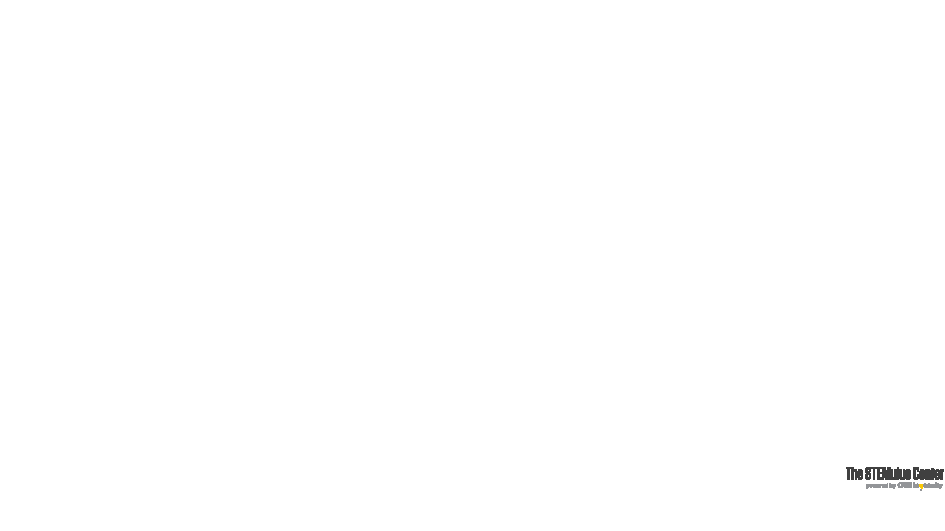
\includegraphics[width=\paperwidth,height=\paperheight]{../artifacts/stemulus.pdf}%
}
\setbeamertemplate{caption}[numbered]
\lstset{%
	breaklines=true,
	captionpos=b,
	frame=single,
	keepspaces=true,
	showstringspaces=false
}

% page numbers
\addtobeamertemplate{navigation symbols}{}{%
    \usebeamerfont{footline}%
    \usebeamercolor[fg]{footline}%
    \hspace{1em}%
    \insertframenumber/\inserttotalframenumber
}

% presentation header
\usetheme{Warsaw}
\title{Agile Development Methodologies}
\author{Dylan Lane McDonald}
\institute{CNM STEMulus Center\\Web Development with PHP}
\date{\today}

\begin{document}
\lstset{language=Java}
\begin{frame}
\titlepage
\end{frame}

\begin{frame}
\frametitle{Outline}
\tableofcontents
\end{frame}

\section{Agile Development Methodologies}
\begin{frame}
\frametitle{Agile Development Methodologies}
\begin{qotd}
``All the world's a stage,\\
And all the men and women merely players:\\
They have their exits and their entrances;\\
And one man in his time plays many parts,\\
His acts being seven ages.''\\
$\approx$ William Shakespeare
\end{qotd}
\pause
\textbf{Agile development methodologies} is an ``umbrella term'' for many different methodologies, all of which are ``agile'' and adapt to changing requirements very fast.
\end{frame}


\subsection{Common Features}
\begin{frame}
\frametitle{Common Features of All Agile Methods}
All agile methodologies have  the following features in common:
\begin{itemize}
	\item \textbf{Iterative}: The development process is done small slices and releases are scheduled regularly
	\item \textbf{Communication}: The product owner is very involved and constantly providing feedback to the development team
	\item \textbf{Quality}: High quality standards are maintained through methods such as continuous integration, unit testing, test-driven development, and refactoring
	\item \textbf{Adaptive}: Software development evolves as new features, bug reports, and client needs are given in the communication cycle  
\end{itemize}
\end{frame}

\subsection{Agile Vocabulary}
\begin{frame}
\frametitle{Agile Actors}
All agile methods have various roles in the development process. Please add all these roles to your lexicon.
\begin{itemize}
	\item \textbf{Product Owner}: The individual who represents the client's interest in the software development process
	\item \textbf{Project Manager\footnote{Also known as a ``master''}}: The individual who supervises the development team, approves sprints, and assigns tasks
	\item \textbf{Developer}: Team member who, in addition to writing software, writes documentation, tests and verifies all units, and provides feedback to the project manager
\end{itemize}
Software teams in an agile environment are self-organizing. Developers organize based on current projects and how their talents are best suited to particular tasks.
\end{frame}

\begin{frame}
\frametitle{Agile Phases}
The agile process consists of various phases. Please add these to your lexicon, too:
\begin{enumerate}
	\item Tickets are taken from the \textbf{backlog}, which is a group of tickets waiting for development
	\item This group of tickets is known as a \textbf{sprint}; the sprint is then given a time limit
	\item Daily \textbf{stand up meetings} designed to keep everyone up to date; these meetings are designed to be only 5 - 10 minutes
	\item As developers complete tickets, they write tests for all their code, known as \textbf{unit tests}
	\item The sprint is then worked on by the developers and the tickets will gradually become complete; the rate at which this happens is known as the \textbf{burn down}
\end{enumerate}
\end{frame}

\section{Different Agile Methodologies}
\begin{frame}
\frametitle{Different Agile Methodologies}
There is no one agile methodology. Organizations will often create ``hybrid'' methods of two or more methodologies. As always, there are advantages and disadvantages to each.
\begin{itemize}
	\item \textbf{Extreme Programming (XP)}: Method where developers use \textbf{pair programming}: one keyboard, two developers
	\item \textbf{Kanban}: Kanban stresses just-in-time delivery and limiting the tickets that are in progress
	\item \textbf{Scrum}: A flexible methodology that emphasizes the ability of the team to adapt to a product that may or may not be well defined
	\item \textbf{Test Driven Development}: A methodology that enforces all unit tests be written before the actual unit
\end{itemize}
\end{frame}

\section{Scrum}
\begin{frame}
\frametitle{Scrum}
\begin{figure}
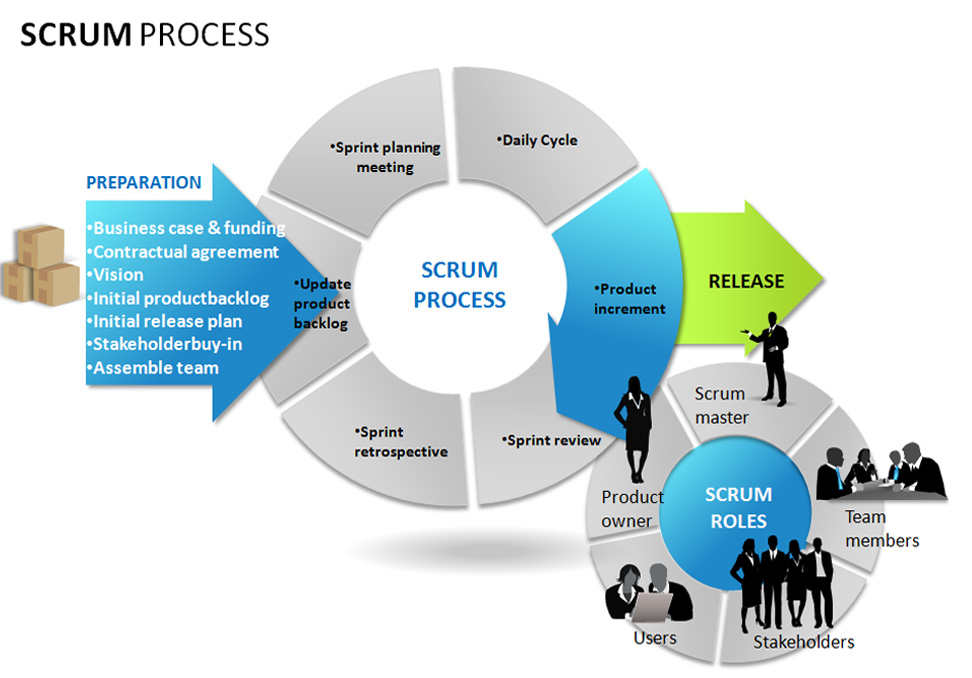
\includegraphics[scale=0.25]{../artifacts/scrum.jpg}
\caption{Scrum Development Process}
\label{fig:scrum}
\end{figure}
\end{frame}

\begin{frame}
\frametitle{In Class Agile}
Like many job sites, this class will be using a ``hybrid'' approach to agile development. Specifically, the following features will be used from the processes discussed:
\begin{itemize}
	\item Roles, stand-up meetings, sprints, and burn downs will be used from Scrum
	\item In progress tickets will be limited as per Kanban
	\item \textbf{All} JavaScript and PHP code must be unit tested before it is written, as is seen in test driven development
\end{itemize}
Essentially, the class will be using Scrum with a few added features from Kanban and test driven development.
\end{frame}
\end{document}